% ===========================================================================
% CS 620 project report -- AAAI Press format
% Compile:  pdflatex report && bibtex report && pdflatex report && pdflatex report
% Replace aaai2026.sty / aaai2026.bst with the official files from the AAAI
% author kit before submission (this folder ships stand-in versions).
% ===========================================================================
\documentclass[letterpaper]{article}
\usepackage{aaai2026}
\usepackage{times}
\usepackage{helvet}
\usepackage{courier}
\usepackage[hyphens]{url}
\usepackage{graphicx}
\urlstyle{rm}
\def\UrlFont{\rm}
\usepackage{natbib}
\usepackage{caption}
\frenchspacing
\setlength{\emergencystretch}{2em}
\setcounter{secnumdepth}{2}
\setlength{\pdfpagewidth}{8.5in}
\setlength{\pdfpageheight}{11in}
\usepackage{amsmath,amssymb}
\usepackage{booktabs}
\usepackage{algorithm}
\usepackage{algorithmic}
\usepackage{xcolor}
\definecolor{linkblue}{RGB}{20,60,140}
\usepackage[colorlinks=true,linkcolor=linkblue,citecolor=linkblue,urlcolor=linkblue]{hyperref}
\newcommand{\TT}{1500}
\newcommand{\Seeds}{3}
\newcommand{\RedRandA}{69}
\newcommand{\RedGPA}{60}
\newcommand{\RedNPA}{27}
\newcommand{\RhoHatHi}{0.82}
\newcommand{\RhoHatMid}{0.52}
\newcommand{\ProbesOFHi}{0.97}
\newcommand{\ProbesSALHi}{0.01}
\newcommand{\RegOFHi}{128.9}
\newcommand{\RegSAKHi}{125.5}
\newcommand{\RegSALHi}{125.3}
\newcommand{\RegNPHi}{123.7}
\newcommand{\RegOFMid}{123.6}
\newcommand{\RegSALMid}{134.6}
\newcommand{\RegLCBMid}{117.9}
\newcommand{\RegLCBHi}{116.2}
\newcommand{\ProbesLCBHi}{0.31}
\newcommand{\ProbesLCBMid}{0.97}
\newcommand{\PointHi}{0.80}
\newcommand{\PointMid}{0.43}
   % numbers generated from results/*.csv by make_tables.py

\newcommand{\NSW}{\mathrm{NSW}}
\newcommand{\E}{\mathbb{E}}
\newcommand{\rhat}{\hat{\rho}}

\title{Reproducing Fair Probing for Multi-Agent Bandits\\ and Making It Robust to Stale Probes}
\author{Korra Prashanth Nayak (Roll No.\ 25210075)}
\affiliations{CS 620: Incentives in Machine Learning, Indian Institute of Technology Gandhinagar\\ korra.nayak@iitgn.ac.in}

\begin{document}
\maketitle

\begin{abstract}
I reproduce the Online Fair Multi-agent UCB with Probing (OFMUP) algorithm of
\citet{xu2026fair}, which combines fair assignment by Nash social welfare (NSW)
with a probing mechanism that inspects a few arms before each round, and I
extend it. My reproduction follows the methodology of the original paper and
makes explicit the modelling choices it leaves open, several of which (an
infeasible capacity constraint when agents outnumber arms, an unspecified
probing cost, and a scale mismatch in Xu et al.'s Algorithm~1) must be resolved before the
method can be run at all. I then address a practical limitation of the model:
it assumes that a probed reward is exactly the reward an agent obtains on
arrival, although in ridesharing demand can change while a driver travels. I
propose Staleness-Aware OFMUP (SA-OFMUP), which models a probability $\rho$ that
a probe is out of date, replaces the raw probe value by its conditional
expectation in both probing and assignment, estimates $\rho$ online from
probe--pull pairs with a ratio estimator that remains consistent under adaptive
assignment under stated conditions (proof sketch), and plans with a lower confidence bound on $\rho$, so that probing
continues until the data show that it is not worthwhile. At $\rho=0$, SA-OFMUP
reduces exactly to OFMUP with the counting fix. Experiments on the same synthetic
settings reproduce the original ranking of methods; under
staleness, SA-OFMUP learns $\rho$ accurately, matches OFMUP at $\rho=0.4$, and has
lower regret than OFMUP on all three seeds at $\rho=0.8$ (about 10\% on average
at $T=1500$ and 14\% at the original horizon $T=3000$; 3 seeds). I also report several
issues in the original paper, including a double counting of probe samples in
Xu et al.'s Algorithm~2 and a simple counterexample to its Lemma~5.
\end{abstract}

\section{Introduction}

In a multi-agent multi-armed bandit (MA-MAB), a central planner assigns $M$
agents to $A$ arms in every round and observes the resulting rewards. The
canonical example is ridesharing, in which the agents are drivers, the arms are
pickup zones and the planner is the dispatcher. Maximising the sum of rewards
can leave some agents with almost nothing (``starvation''), so a line of work
replaces the sum by the Nash social welfare (NSW), the product of the agents'
utilities
\citep{kaneko1979nash,caragiannis2019unreasonable,hossain2021fair,jones2023efficient}.
\citet{xu2026fair} add \emph{probing}: before assigning, the planner may pay to
observe fresh rewards on a few arms. They give an offline greedy probing
algorithm with a constant-factor guarantee and an online algorithm, OFMUP, with
sublinear regret. Prior work on probing, such as Observe-Before-Play bandits \citep{zuo2020observe} and bandits with costly probes \citep{elumar2024costly}, assumes that a probed reward remains valid when the arm is played; SA-OFMUP relaxes this assumption by modelling probes that go stale before an agent arrives and learning the staleness rate online within fair NSW-based assignment.

This project has two goals: to reproduce the methodology and results of
\citet{xu2026fair} as faithfully as possible, and to extend the method in one
substantive direction. My contributions are as follows.
\begin{enumerate}
  \item An independent implementation of OFMUP, its three baselines and the
        regret benchmark, with every open modelling choice documented
        (Section~\ref{sec:repro}).
  \item A critical reading of \citet{xu2026fair} that identifies problems a
        reproduction cannot avoid: the capacity constraint is infeasible in
        its own experiments, lines 9 and 11 of Xu et al.'s Algorithm~1 compare
        quantities on different scales, Xu et al.'s Algorithm~2 counts some samples
        twice, and Lemma~5 admits a two-agent counterexample
        (Section~\ref{sec:findings}).
  \item SA-OFMUP, a staleness-aware extension with an exact conditional-mean
        objective, an online estimator of the staleness rate, and a proof
        sketch of its consistency (Section~\ref{sec:sa}).
  \item Experiments that reproduce the qualitative results of the original
        paper and evaluate SA-OFMUP under increasing staleness
        (Section~\ref{sec:exp}).
\end{enumerate}
The code is provided with this report: the single notebook-cell script
\texttt{final\_one\_cell.py} reruns every experiment and regenerates every figure
and the data behind every table.

\section{Background and Problem Setting}

\subsection{Agents, arms and rewards}
There are $M$ agents and $A$ arms. Each pair $(j,a)$ has an unknown reward
distribution $D_{j,a}$ on $[0,1]$ with mean $\mu_{j,a}$. Each round $t$ has three
steps. First, the planner selects a \emph{probing set} $S_t\subseteq[A]$ and
observes a fresh sample $R_{j,a,t}\sim D_{j,a}$ for every agent $j$ and every
$a\in S_t$. Second, it chooses an assignment policy $\pi_t$. Third, each agent
$j$ pulls an arm $a_{j,t}\sim\pi_t$ and observes its reward.

\subsection{Nash social welfare}
For an assignment $\pi$, the expected utility of agent $j$ is $u_j=\sum_a
\pi_{j,a}\,r_{j,a}$, where $r_{j,a}$ is the fresh sample for probed arms and the
mean $\mu_{j,a}$ otherwise. The objective is the product of utilities,
\begin{equation}
  \NSW(S,R,\mu,\pi)=\prod_{j\in[M]}\Big(\sum_{a\in S}\pi_{j,a}R_{j,a}+\sum_{a\notin S}\pi_{j,a}\mu_{j,a}\Big).
  \label{eq:nsw}
\end{equation}
NSW is Pareto efficient and scale invariant, and lies between the utilitarian
sum and max--min fairness \citep{caragiannis2019unreasonable}. Following the
experiments of \citet{xu2026fair}, I report the geometric mean $\NSW^{1/M}$,
which has the same maximiser.

\subsection{Probing cost and regret}
Probing $|S|$ arms costs a fraction $\alpha(|S|)$ of the round's value, where
$\alpha$ is non-decreasing with $\alpha(0)=0$ and $\alpha(I)=1$ for a budget $I$.
The value of round $t$ is then
$R^{\mathrm{total}}_t=(1-\alpha(|S_t|))\,\E_{R_t}[\NSW(S_t,R_t,\mu,\pi_t)]$. The
benchmark is the offline optimum $(S^\ast,\pi^\ast)$ computed with full
knowledge of $\mu$, and the cumulative regret is
\begin{equation}
  \mathcal{R}(T)=\sum_{t=1}^T\Big[(1-\alpha(|S^\ast|))\,\E\big[\NSW(S^\ast,R_t,\mu,\pi^\ast)\big]-R^{\mathrm{total}}_t\Big].
  \label{eq:regret}
\end{equation}

\subsection{The OFMUP Framework}
\textbf{Xu et al.'s Algorithm 1 (offline greedy probing)} first builds a greedy chain
$S_0=\emptyset\subset S_1\subset\dots\subset S_I$, each step adding the arm with
the largest gain in a surrogate $f_{\mathrm{upper}}(S)=\phi(g(S))$, where $g(S)$
is the best NSW achievable using only probed arms and $\phi$ is a
piecewise-linear upper envelope of $\log$ built from tangent lines. It then
ranks the candidates by $(1-\alpha(|S_j|))f_{\mathrm{upper}}(S_j)$ and applies
two checks before returning one of them. Theorem~1 of \citet{xu2026fair}
guarantees
$\mathcal{R}(S^{\mathrm{pr}})\ge\frac{e-1}{2e-1}\cdot\frac1\zeta\,\mathcal{R}(S^\ast)\approx 0.387\,\mathcal{R}(S^\ast)/\zeta$.
\textbf{Xu et al.'s Algorithm 2 (OFMUP)} maintains empirical distributions $\hat F_{j,a}$,
means $\hat\mu_{j,a}$ and upper confidence bounds
$U_{j,a}=\min(\hat\mu_{j,a}+w_{j,a},1)$ with the empirical-Bernstein bonus of
Lemma~7 \citep{maurer2009empirical}. After a warm start of $MA$ rounds, each
round calls Xu et al.'s Algorithm~1 on $\hat F$, probes, updates the statistics, assigns by
maximising $(1-\alpha(|S_t|))\E[\NSW(S_t,R_t,U_t,\pi_t)]$, pulls, and updates
the statistics again. Theorem~2 gives regret
$O\big(\zeta(\sqrt{MAT}+MA)\ln^c(MAT/\delta)\big)$.

\section{Reproduction Methodology}
\label{sec:repro}

I implemented the simulator, the NSW solver, both algorithms and the three
baselines in NumPy. Running the method requires settling several points that
the original paper does not specify; Table~\ref{tab:choices} lists them, and I
discuss the three most consequential below.

\begin{table}[t]
\centering\small
\begin{tabular}{p{0.3\columnwidth}p{0.62\columnwidth}}
\toprule
Open point & My choice \\
\midrule
Assignment constraints: rows of $\pi$ sum to 1, columns $\le 1$; infeasible when $M>A$ (all four experimental settings) & Each agent has its own row; each arm receives at most $M/A$ agents in expectation. A ``shared'' policy $\pi\in\Delta^A$ \citep{jones2023efficient} is also implemented. \\
Overhead $\alpha$ not given & $\alpha(k)=(k/I)^3$ with $I=4$; satisfies $\alpha(0)=0$, $\alpha(I)=1$, non-decreasing. \\
Xu et al.'s Algorithm 1, lines 9 and 11 compare $f_{\mathrm{upper}}$ (log scale, $\le 0$) with $h(\emptyset)$ and $\mathcal{R}(S_j)$ (NSW scale, $\ge 0$) & Keep the greedy chain (lines 1--5); return the chain set with the largest Monte Carlo estimate of $\mathcal{R}(S_j)$, including $S_0=\emptyset$. \\
NSW aggregation & Geometric mean, as in the original experiments. \\
$\hat F_{j,a}\leftarrow 1$ ``optimistic'' initialisation & Point mass at reward 1. \\
Warm-start rounds (one agent acts) & Not counted in regret. \\
Discrete-reward distribution & Random (Dirichlet) weights on $\{0.3,\dots,0.8\}$. \\
Optimal assignment given $S$ & Multiplicative (EM-style) ascent on $\sum_j\log u_j$ with capacity rescaling, 60 iterations. \\
\bottomrule
\end{tabular}
\caption{Modelling choices required to run the method of \citet{xu2026fair}, that are not specified in their paper.}
\label{tab:choices}
\end{table}

\paragraph{Capacity.}
\citet{xu2026fair} require $\sum_j\pi_{j,a,t}\le1$ for every arm, yet its
experiments use $M=12,A=8$ and $M=20,A=10$, for which no feasible $\pi$ exists
(the total mass $M$ exceeds $A$). I relax the capacity to $M/A$ agents per arm.
This preserves the intent of the constraint (no arm is over-used relative to
its share) and reduces to the original constraint when $M=A$.

\paragraph{Xu et al.'s Algorithm 1, Phase 2.}
$f_{\mathrm{upper}}=\phi(g)$ approximates $\log g\le0$, whereas $h(\emptyset)$ and
$\mathcal{R}(S_j)$ are NSW values in $[0,1]$; the comparisons in lines 9 and 11
therefore cannot be executed as written. Since these lines serve to select a
candidate with a good true value, I evaluate $\mathcal{R}(S_j)$ by Monte Carlo
for all $I+1$ candidates and return the best, with
$\mathcal{R}(\emptyset)=h(\emptyset)$ (no probing). The greedy chain itself is
kept exactly as specified. Moreover, $\phi$ is strictly increasing,
so the greedy order is the order of $g$ itself: $\phi$ affects the proof of
Theorem~1 but not the arms that the algorithm selects.

\paragraph{Benchmark.}
As in \citet{xu2026fair}, the optimum is found by exhaustive search over all
probing sets with $|S|\le I$; the expectation over probe outcomes is estimated
from 300 Monte Carlo draws, with the assignment re-optimised for each draw. I
verified the benchmark: an oracle that knows $\mu$ and uses the optimal probing
set achieves zero average regret, whereas the same oracle without probing
incurs positive regret in every round.

\section{SA-OFMUP: Staleness-Aware Probing}
\label{sec:sa}

\subsection{Motivation}
Equation~\eqref{eq:nsw} treats the probed value $R_{j,a,t}$ as the reward that
agent $j$ will obtain if assigned to arm $a$ in the same round. In ridesharing
this is optimistic: the dispatcher checks the demand in a zone, but the driver
needs time to get there, and some of the observed requests will have been
served in the meantime. OFMUP therefore has two weaknesses. First, it trusts a
probe that may be out of date when assigning. Second, it pays the probing cost
for information that is only partly useful.

\subsection{Staleness model}
With probability $\rho\in[0,1]$, independently for each arm and round and
\emph{independently of the probed value}, a probed arm goes stale: an agent
assigned to it obtains a fresh draw from $D_{j,a}$ instead of the probed value.
With probability $1-\rho$ the probe remains valid. Agents assigned to unprobed
arms always receive a fresh draw, as in OFMUP. Setting $\rho=0$
recovers the original model exactly.

\subsection{Objective and assignment}
For a probed pair, the conditional expectation of the obtained reward is
\begin{equation}
  \E[Y_{j,a}\mid R_{j,a}]=(1-\rho)R_{j,a}+\rho\,\mu_{j,a}.
  \label{eq:condexp}
\end{equation}
I define the staleness-aware objective by substituting \eqref{eq:condexp} into
\eqref{eq:nsw}:
\begin{equation}
  \NSW_{\rho}=\prod_{j}\Big(\sum_{a\in S}\pi_{j,a}\big[(1-\rho)R_{j,a}+\rho\mu_{j,a}\big]+\sum_{a\notin S}\pi_{j,a}\mu_{j,a}\Big).
\end{equation}
Like \eqref{eq:nsw}, this is a product of each agent's \emph{expected} utility,
so the substitution is exact by linearity of expectation alone. No independence
between agents is required, and the substitution remains exact when a single
staleness event affects all agents assigned to the same arm. (It differs from
$\E[\prod_j Y_j]$, which is not the original objective either.)
Online, the unknown $\mu_{j,a}$ in \eqref{eq:condexp} is replaced by the same
optimistic estimate $U_{j,a}$ that OFMUP already uses for unprobed arms, and
$\rho$ by its estimate $\rhat$:
$\tilde r_{j,a}=(1-\rhat)R_{j,a}+\rhat\,U_{j,a}$. Inside Xu et al.'s Algorithm~1 the stale
part uses the mean of $\hat F_{j,a}$, which is the value Xu et al.'s Algorithm~1 uses for
unprobed arms. The transform shrinks probe outcomes towards their mean, so the
estimated value of probing decreases with $\rhat$ and the ``no probing''
candidate is selected more often: SA-OFMUP probes less when probes are stale,
without any additional rule.

\subsection{Learning the staleness rate}
If agent $j$ is assigned to a probed arm $a$, both the probe $X=R_{j,a,t}$ and the
obtained reward $Y$ are observed. Under the model,
$\E[X-Y\mid X]=\rho\,(X-\mu_{j,a})$ for every value of $X$, which suggests the
ratio estimator
\begin{equation}
  \rhat=\frac{\sum_i (X_i-Y_i)}{\sum_i (X_i-\hat\mu_i)},
  \label{eq:rhohat}
\end{equation}
computed over all probe--pull pairs $i$ observed so far, clipped to $[0,1]$, and
used only once the denominator exceeds a threshold $\kappa=5$ (until then
$\rhat=0$ and SA-OFMUP behaves as OFMUP). Because the relationship holds
conditionally on $X$, selecting pairs on the basis of the probe value does not
bias the estimator.

\paragraph{Consistency sketch.}
Let $D_i=(X_i-Y_i)-\rho(X_i-\mu_i)$. Whether pair $i$ is selected depends only
on past data and the current probes, while the staleness event and the fresh
draw are independent of both; hence $\E[D_i\mid\mathcal{F}_{i}]=0$ and $|D_i|\le2$,
so $(D_i)$ is a bounded martingale difference sequence. Rearranging
\eqref{eq:rhohat},
\begin{equation*}
  \rhat-\rho=\frac{\sum_i D_i+\rho\sum_i(\hat\mu_i-\mu_i)}{\sum_i(X_i-\hat\mu_i)} .
\end{equation*}
By the Azuma--Hoeffding inequality \citep{azuma1967weighted},
$|\sum_i D_i|=O(\sqrt{n\log(1/\delta)})$ with probability $1-\delta$, and
$|\hat\mu_i-\mu_i|\le w_i$ on the event of Lemma~7. If the denominator grows
linearly in $n$, which happens whenever the selected probes are systematically
above the mean, then $\rhat\to\rho$.

\paragraph{Two implementation details.}
First, $\hat\mu_i$ in \eqref{eq:rhohat} must be the \emph{current} mean, computed
from all data observed so far. Using the mean estimated before the round instead
makes $\rhat$ far too high ($\approx0.95$ for $\rho=0.6$): arms are probed
because their estimated means are high, so the denominator is systematically
too small.

Second, the point estimate must not be used directly for planning, because of a
\emph{lock-in} feedback loop: probe--pull pairs are generated only while the
planner probes. If a noisy early $\rhat$ is high enough to stop probing, no new
pairs arrive and the estimate can never correct itself.
Table~\ref{tab:lockin} shows this effect on the three seeds at $\rho=0.4$:
seed~1 formed $\rhat\approx0.72$ from its first 14 pairs, stopped probing at
round 134, and remained frozen near that value (0.71 at the end;
Table~\ref{tab:lockin}), while the other two seeds kept probing
and converged to $0.41$--$0.44$. The seed average ($0.52$) therefore reflects
one locked-in run rather than a biased estimator.

\paragraph{Planning with a lower confidence bound.}
Probes are trusted until the data show that they are stale. The planner uses
\begin{equation}
  \rho_{\mathrm{LCB}}=\mathrm{clip}\Big(\frac{\sum_i(X_i-Y_i)-c\sqrt{n}}{\sum_i(X_i-\hat\mu_i)},\,0,\,1\Big),
  \label{eq:lcb}
\end{equation}
where $n$ is the number of pairs. The $\sqrt n$ term is the Azuma--Hoeffding
width from the consistency sketch. The constant $c=1$ is a heuristic width of
the same order as the Azuma--Hoeffding width in the sketch; it was fixed before
the experiments rather than tuned. Equation~\eqref{eq:lcb} is therefore a
heuristic bound, not a proven $(1-\delta)$ confidence bound. Early on,
$\rho_{\mathrm{LCB}}=0$ and SA-OFMUP behaves exactly as OFMUP with the counting
fix (OFMUP+fix; Section~\ref{sec:count}); it discounts probes only once many
pairs confirm staleness, by which time the point estimate is accurate. I denote
this version SA-OFMUP (LCB, final) and use it as the proposed method; the version
that plans with the point estimate, SA-OFMUP (point estimate), is retained as an
ablation.

\begin{table}[t]
\centering\small
\begin{tabular}{lccc}
\toprule
Seed ($\rho=0.4$) & Final $\rhat$ & Probes/round & Last probe \\
\midrule
0 & 0.41 & 0.48 & round 1499 \\
1 & 0.71 & 0.01 & round 134 (locked) \\
2 & 0.44 & 0.97 & round 1499 \\
\bottomrule
\end{tabular}
\caption{Lock-in of SA-OFMUP (point estimate) at $\rho=0.4$ (setting (a), $T=\TT$): seed~1 stopped probing early on a noisy estimate and could never revise it.}
\label{tab:lockin}
\end{table}

\subsection{Counting fix}
\label{sec:count}
In Xu et al.'s Algorithm~2 a probed arm's sample is recorded at line~13; if an agent is
then assigned to that arm, line~16 records the pull as well. At $\rho=0$ the pull
\emph{is} the probed draw, so the same sample is counted twice and the
confidence bonus shrinks faster than the data warrant. SA-OFMUP records the
probe only and uses the pair solely for \eqref{eq:rhohat}. To separate the
effect of this fix from the staleness mechanism, I also evaluate OFMUP+fix,
which is OFMUP with only this change. Algorithm~\ref{alg:sa} lists the full
procedure; lines marked $\star$ differ from the original algorithm.

\setcounter{algorithm}{2}
\begin{algorithm}[t]
\caption{SA-OFMUP (changes to Xu et al.'s Algorithm~2 marked $\star$)}
\label{alg:sa}
\begin{algorithmic}[1]
\STATE Initialise $\hat F,N,\hat\mu,w$ as in OFMUP; $\mathrm{num}\leftarrow0$, $\rhat\leftarrow0$ $\star$
\STATE Warm start for $t=1,\dots,MA$ as in OFMUP
\FOR{$t=MA+1,\dots,T$}
  \STATE $S_t\leftarrow{}$Xu et al.'s Algorithm~1$(\hat F,\alpha,I,\rhat)$ with transform $(1-\rhat)x+\rhat\,\bar F$ $\star$
  \STATE Probe $S_t$, observe $X_{j,a}$, update $\hat F,N,\hat\mu,w,U$
  \STATE $\tilde r_{j,a}\leftarrow(1-\rhat)X_{j,a}+\rhat\,U_{j,a}$ for $a\in S_t$; $\tilde r_{j,a}\leftarrow U_{j,a}$ otherwise $\star$
  \STATE $\pi_t\leftarrow\arg\max_\pi(1-\alpha(|S_t|))\prod_j\sum_a\pi_{j,a}\tilde r_{j,a}$
  \STATE Each agent pulls $a_{j}\sim\pi_{t}$ and observes $Y_j$
  \FOR{each agent $j$}
    \IF{$a_j\in S_t$}
      \STATE $\mathrm{num}\mathrel{+}=X_{j,a_j}-Y_j$;\; record the pair $(j,a_j,X_{j,a_j})$; do \emph{not} re-count the sample $\star$
    \ELSE
      \STATE update $\hat F,N,\hat\mu,w,U$ with $Y_j$
    \ENDIF
  \ENDFOR
  \STATE $\mathrm{den}\leftarrow\sum_{\text{pairs}}(X-\hat\mu_{\text{current}})$;\; $\rhat\leftarrow\mathrm{clip}\big((\mathrm{num}-c\sqrt{n})/\mathrm{den},0,1\big)$ if $\mathrm{den}\ge\kappa$ else $0$, where $n$ is the number of probe--pull pairs $\star$ (Eq.~\ref{eq:lcb})
\ENDFOR
\end{algorithmic}
\end{algorithm}

\section{Experiments}
\label{sec:exp}

\subsection{Setup}
I follow the experimental setup of \citet{xu2026fair}: $M=12,A=8$ (small) and $M=20,A=10$ (medium);
Bernoulli rewards with means in $[0.3,0.8]$ and discrete rewards on
$\{0.3,\dots,0.8\}$; budget $I=4$; and $\delta=0.1$. Owing to compute limits,
the sweeps use $T=\TT$ rounds and $\Seeds$ seeds, with a new problem instance per
seed; setting (a) at $\rho=0$ and the $\rho=0.8$ test were also run at the
original horizon $T=3000$ (Tables~\ref{tab:repro3000} and \ref{tab:long},
Figure~\ref{fig:long}). The baselines are the same three as in the original study:
Non-Probing \citep{jones2023efficient}, Random P+A (random probes and uniform
random assignment) and Greedy P+A (Xu et al.'s Algorithm~1 probes with random assignment).
Regret is computed against the exhaustive-search optimum of the \emph{true}
model (true $\mu$ and $\rho$), and every method's decisions are scored with the
true parameters, never with its own estimates. Curves show the mean over seeds
with one standard deviation shaded.

\subsection{Reproduction Results}

\begin{figure*}[t]
\centering
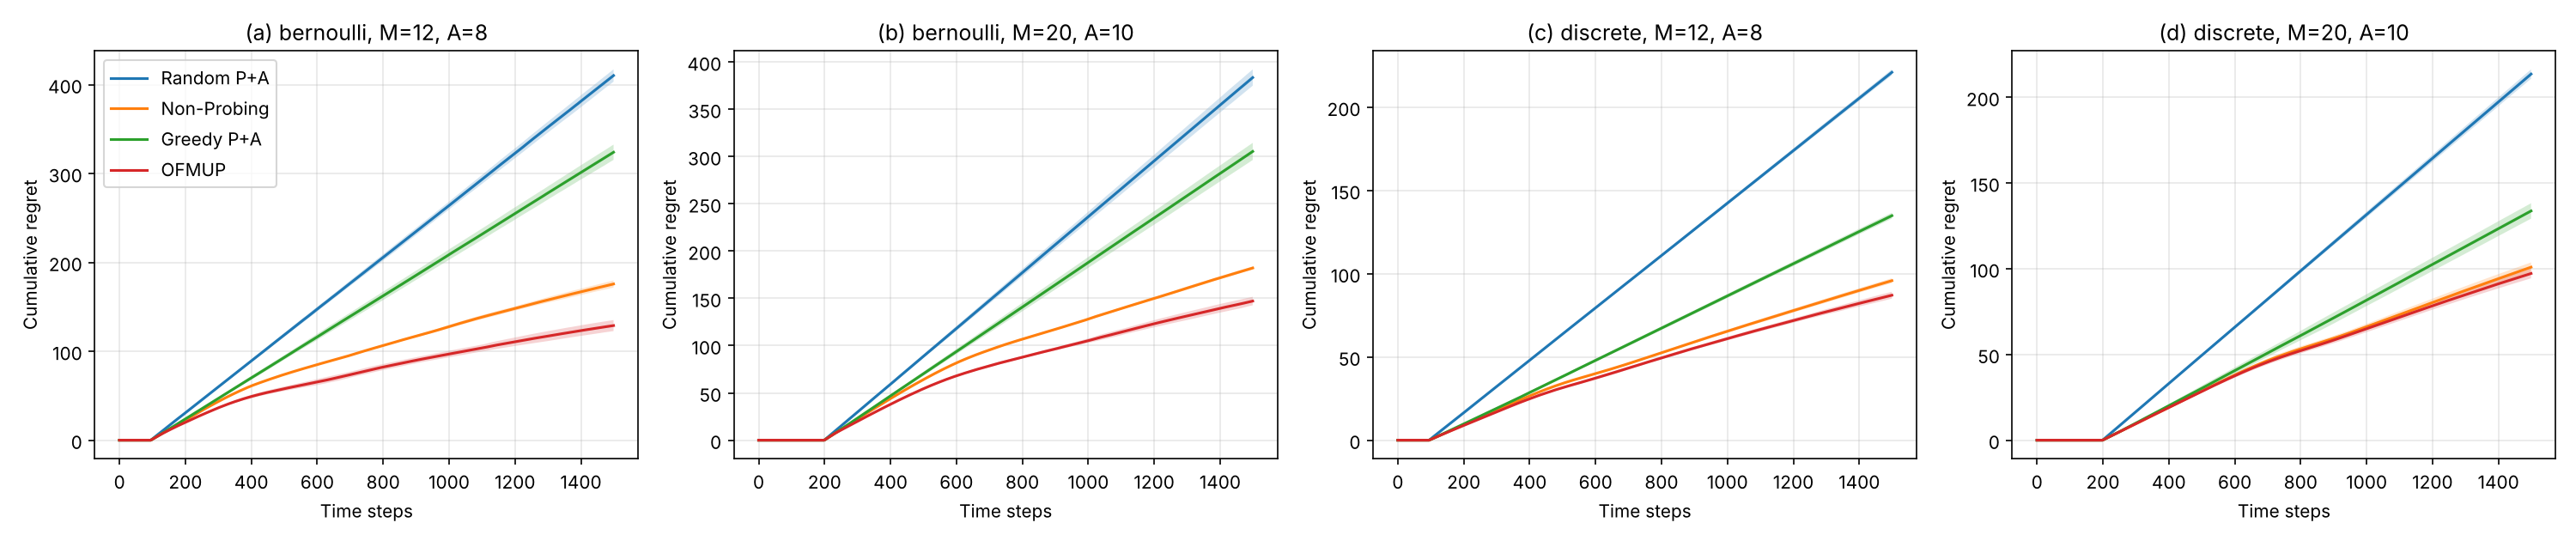
\includegraphics[width=\textwidth]{results/fig1_reproduction.png}
\caption{Cumulative regret at $\rho=0$ in the four settings of Figure~1 of
\citet{xu2026fair} ($T=\TT$, \Seeds{} seeds). (a) Bernoulli, $M=12,A=8$; (b) Bernoulli,
$M=20,A=10$; (c) discrete, $M=12,A=8$; (d) discrete, $M=20,A=10$. The flat
stretch at the start is the warm start of $MA$ rounds, during which only one
agent acts and no regret is counted (Table~\ref{tab:choices}).}
\label{fig:repro}
\end{figure*}

\begin{table*}[t]
\centering\small
\begin{tabular}{lrrrr}
\toprule
Setting & Random P+A & Greedy P+A & Non-Probing & OFMUP \\
\midrule
(a) bern., $M$=12, $A$=8 & 410.2 $\pm$ 6.9 & 323.9 $\pm$ 8.6 & 175.7 $\pm$ 4.0 & 128.9 $\pm$ 6.2 \\
\quad OFMUP reduction & 69\% & 60\% & 27\% & - \\
(b) bern., $M$=20, $A$=10 & 383.5 $\pm$ 8.6 & 305.4 $\pm$ 9.1 & 182.1 $\pm$ 1.6 & 147.1 $\pm$ 4.5 \\
\quad OFMUP reduction & 62\% & 52\% & 19\% & - \\
(c) disc., $M$=12, $A$=8 & 221.0 $\pm$ 1.7 & 134.9 $\pm$ 1.8 & 95.8 $\pm$ 1.5 & 87.1 $\pm$ 2.0 \\
\quad OFMUP reduction & 61\% & 35\% & 9\% & - \\
(d) disc., $M$=20, $A$=10 & 213.6 $\pm$ 2.7 & 133.7 $\pm$ 4.5 & 100.9 $\pm$ 2.8 & 97.2 $\pm$ 2.8 \\
\quad OFMUP reduction & 54\% & 27\% & 4\% & - \\
\bottomrule
\end{tabular}

\caption{Final cumulative regret (mean $\pm$ s.d.\ over seeds) at $T=\TT$, and
OFMUP's reduction relative to each baseline. \citet{xu2026fair} report
reductions of 85\%/60\% (vs.\ Random P+A/Greedy P+A) in setting (a) and
88\%/80\% in (b) at $T=3000$; Table~\ref{tab:repro3000} gives the like-for-like
comparison at $T=3000$.}
\label{tab:repro}
\end{table*}

Figure~\ref{fig:repro} and Table~\ref{tab:repro} show that the original qualitative
findings are reproduced: Random P+A is worst, Greedy P+A
is next, and OFMUP has the lowest mean regret in all four settings, although in (d) its
margin over Non-Probing is within the seed-to-seed variation, with Non-Probing
between Greedy P+A and OFMUP. In setting (a), OFMUP's regret is \RedRandA\%
lower than that of Random P+A, \RedGPA\% lower than that of Greedy P+A and
\RedNPA\% lower than that of Non-Probing. At this horizon the reductions are
smaller than those reported by the authors. At the original horizon
$T=3000$ (Table~\ref{tab:repro3000} and Figure~\ref{fig:long}, left), the
reductions in setting (a) are 76\% vs.\ Random P+A, 70\% vs.\ Greedy P+A and
32\% vs.\ Non-Probing. Against Random P+A this is closer to the reported 85\%;
against Greedy P+A, the reduction is 60\% at $T=\TT$ and 70\% at $T=3000$,
against 60\% reported at $T=3000$. I suspect the remaining differences stem from the modelling
choices in Table~\ref{tab:choices}, in particular the overhead function, which
directly controls how often probing pays off. In setting (b) the reductions
(62\% and 52\%) are further below the reported 88\% and 80\%; I did not rerun
(b) at $T=3000$, so I cannot separate the horizon effect from the modelling
choices in Table~\ref{tab:choices}.

\begin{table}[t]
\centering\footnotesize\setlength{\tabcolsep}{4pt}
\begin{tabular}{lrrrr}
\toprule
Setting (a), $T=3000$ & s0 & s1 & s2 & mean $\pm$ s.d. \\
\midrule
Random P+A & 829.2 & 856.9 & 860.7 & 848.9 $\pm$ 14.0 \\
Greedy P+A & 645.4 & 679.7 & 683.7 & 669.6 $\pm$ 17.2 \\
Non-Probing & 302.3 & 284.2 & 312.6 & 299.7 $\pm$ 11.7 \\
OFMUP & 209.7 & 193.3 & 207.9 & 203.6 $\pm$ 7.3 \\
\bottomrule
\end{tabular}
\caption{Final cumulative regret in setting (a) at the original horizon $T=3000$ (3 seeds). OFMUP's reduction: 76\% vs.\ Random P+A, 70\% vs.\ Greedy P+A, 32\% vs.\ Non-Probing.}
\label{tab:repro3000}
\end{table}

The comparison between Greedy P+A and Non-Probing is instructive: probing
without fair assignment is clearly worse than fair assignment without probing,
so the two ingredients are complementary rather than interchangeable, as the
authors argue. OFMUP+fix and OFMUP are within noise of each other at
$\rho=0$ (Table~\ref{tab:stale}): at this horizon the double counting has no
measurable effect on regret, although it does make the confidence bonuses
smaller than the data justify.

\subsection{Results under Staleness}

\begin{figure*}[t]
\centering
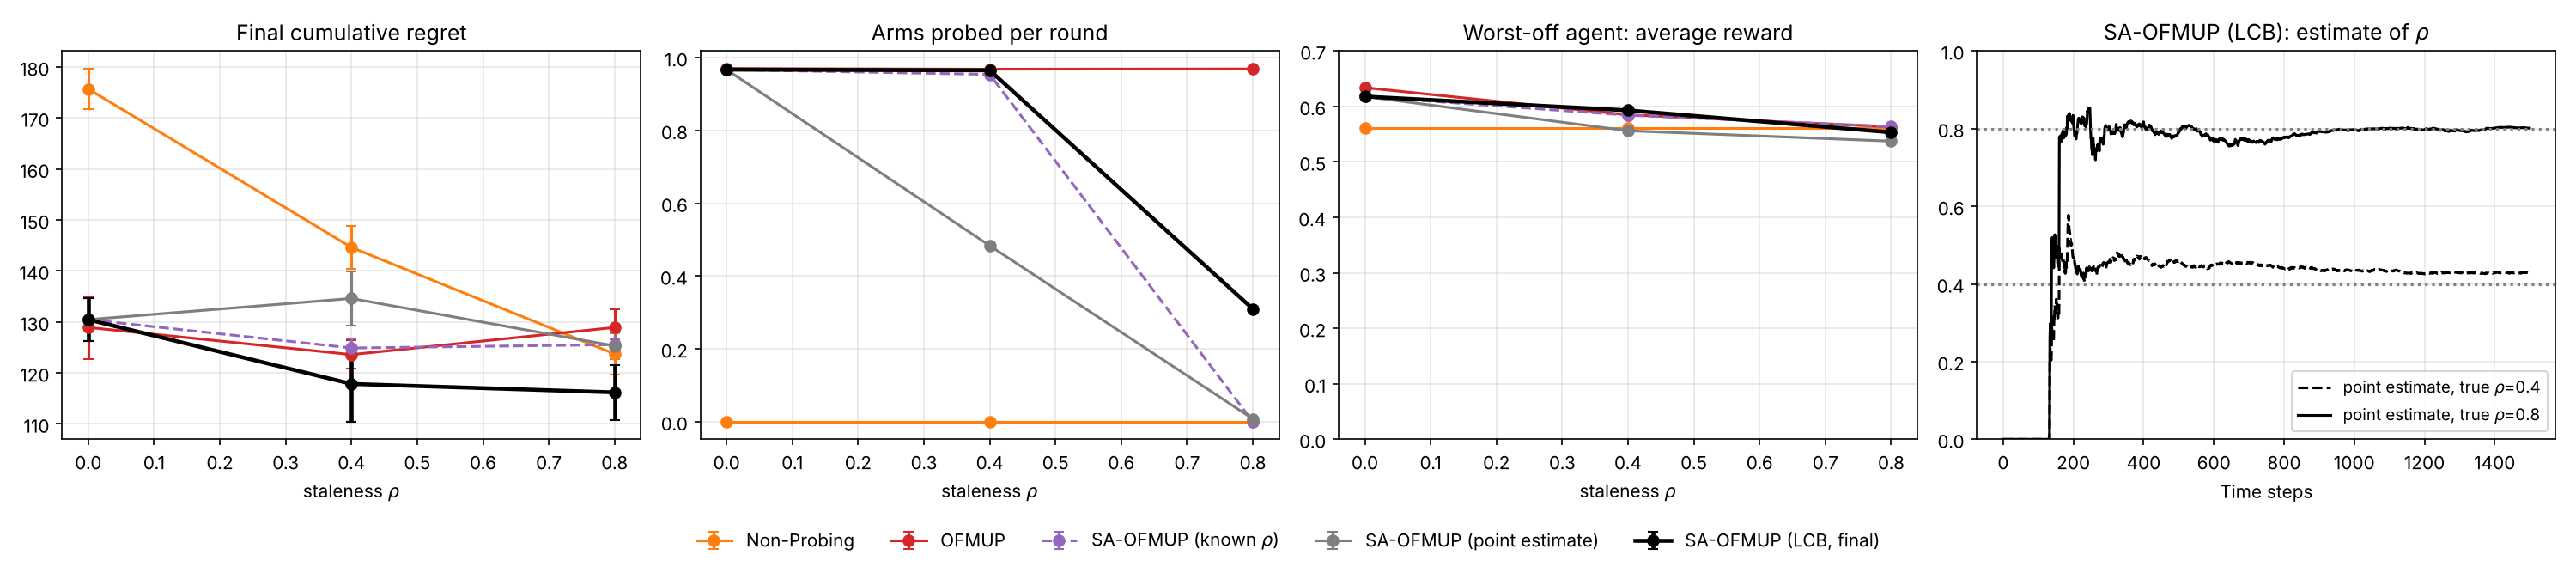
\includegraphics[width=\textwidth]{results/staleness_a.png}
\caption{Staleness sweep in setting (a), $T=\TT$, \Seeds{} seeds. Left to right:
final regret (mean $\pm$ s.d.); arms probed per round; the worst-off agent's
average reward; and the point estimate of $\rho$ over time for SA-OFMUP (LCB,
final), with the true values dotted. OFMUP+fix is omitted from the plots
because it is indistinguishable from OFMUP; its values are given in
Table~\ref{tab:stale}.}
\label{fig:stale}
\end{figure*}

\begin{table}[t]
\centering\footnotesize\setlength{\tabcolsep}{3.5pt}
\begin{tabular}{lrrr}
\toprule
Method & $\rho=0$ & $\rho=0.4$ & $\rho=0.8$ \\
\midrule
\multicolumn{4}{l}{\emph{Final cumulative regret (mean $\pm$ s.d.)}} \\
Non-Probing & 175.7 $\pm$ 4.0 & 144.6 $\pm$ 4.2 & 123.7 $\pm$ 4.1 \\
OFMUP & 128.9 $\pm$ 6.2 & 123.6 $\pm$ 2.8 & 128.9 $\pm$ 3.5 \\
OFMUP+fix & 130.5 $\pm$ 4.2 & 122.5 $\pm$ 1.9 & 126.4 $\pm$ 1.1 \\
SA-OFMUP (known $\rho$) & 130.5 $\pm$ 4.2 & 124.9 $\pm$ 1.9 & 125.5 $\pm$ 1.0 \\
SA-OFMUP (point estimate) & 130.5 $\pm$ 4.2 & 134.6 $\pm$ 5.3 & 125.3 $\pm$ 2.6 \\
\textbf{SA-OFMUP (LCB, final)} & 130.5 $\pm$ 4.2 & 117.9 $\pm$ 7.4 & 116.2 $\pm$ 5.4 \\
\midrule
\multicolumn{4}{l}{\emph{Arms probed per round}} \\
OFMUP & 0.97 & 0.97 & 0.97 \\
OFMUP+fix & 0.97 & 0.97 & 0.97 \\
SA-OFMUP (known $\rho$) & 0.97 & 0.95 & 0.00 \\
SA-OFMUP (point estimate) & 0.97 & 0.48 & 0.01 \\
\textbf{SA-OFMUP (LCB, final)} & 0.97 & 0.97 & 0.31 \\
\midrule
\multicolumn{4}{l}{\emph{Final estimate of $\rho$}} \\
SA-OFMUP (point estimate) & 0.00 & 0.52 & 0.82 \\
SA-OFMUP (LCB), point estimate & 0.00 & 0.43 & 0.80 \\
\bottomrule
\end{tabular}

\caption{Staleness sweep in setting (a), $T=\TT$, \Seeds{} seeds: final regret,
arms probed per round and final estimate of $\rho$ for each method as the true
staleness $\rho$ grows.}
\label{tab:stale}
\end{table}

Table~\ref{tab:stale} and Figure~\ref{fig:stale} report the sweep over $\rho$,
and Table~\ref{tab:seeds} reports every seed. Four observations stand out.
First, at $\rho=0$ all SA-OFMUP variants coincide with OFMUP+fix \emph{exactly}
(identical regret curves for identical seeds), as intended by design. Second,
the point estimate of $\rho$ in SA-OFMUP (LCB, final) is accurate (seed
means $\PointMid$ at $\rho=0.4$ and $\PointHi$ at $\rho=0.8$; Table~\ref{tab:long}
gives per-seed values for $\rho=0.8$ at $T=3000$), so the lock-in did not occur
in these seeds. Third, at $\rho=0.4$ SA-OFMUP (LCB,
final) matches OFMUP: it probes as often (\ProbesLCBMid{} arms per round), and
two of the three seeds are within two regret points of OFMUP. Its lower mean
(\RegLCBMid{} vs.\ \RegOFMid) is driven by a single seed and is therefore not
evidence of an improvement; the result at $\rho=0.4$ is that discounting probes
costs nothing while probing is still worthwhile. SA-OFMUP (point estimate), by
contrast, locks in on one seed (Table~\ref{tab:lockin}), halves its probing on
average, and has a regret (\RegSALMid) clearly above that of OFMUP. Fourth, at
$\rho=0.8$ SA-OFMUP (LCB, final) has lower regret than OFMUP on all three seeds
(\RegLCBHi{} vs.\ \RegOFHi{} on average, about 10\%), and is also below
Non-Probing (\RegNPHi) and SA-OFMUP (known $\rho$) (\RegSAKHi).

I now examine the source of this gain. At $T=\TT$ the planner's lower bound is
still $0.65$--$0.69$, below the true value $0.8$, and SA-OFMUP (LCB, final)
still probes $0.22$--$0.38$ arms per round, whereas SA-OFMUP (known $\rho$)
probes none and merely matches Non-Probing. The advantage over SA-OFMUP (known
$\rho$) therefore does not come from learning $\rho$ and stopping. My
hypothesis is that the conservative bound keeps some probing going, and that
these probes, although mostly stale, still speed up learning of the means; the
bound thus acts as an exploration bonus that Xu et al.'s Algorithm~1 otherwise lacks. If
this hypothesis holds, the advantage over SA-OFMUP (known $\rho$) should not
grow with the horizon: once the evidence of staleness has accumulated and
probing stops, there is no further benefit to collect. A run at $\rho=0.8$ with
$T=3000$ (Section~\ref{sec:long}) tests this prediction.

\begin{table}[t]
\centering\footnotesize\setlength{\tabcolsep}{4pt}
\begin{tabular}{lrrrrrr}
\toprule
 & \multicolumn{3}{c}{$\rho=0.4$} & \multicolumn{3}{c}{$\rho=0.8$} \\
Method & s0 & s1 & s2 & s0 & s1 & s2 \\
\midrule
Non-Probing & 150.0 & 139.8 & 144.1 & 129.5 & 120.1 & 121.6 \\
OFMUP & 126.2 & 124.9 & 119.7 & 127.3 & 133.8 & 125.6 \\
SA-OFMUP (known $\rho$) & 122.5 & 125.2 & 127.0 & 124.8 & 124.9 & 126.9 \\
SA-OFMUP (LCB, final) & 124.9 & 107.6 & 121.0 & 117.1 & 109.2 & 122.3 \\
\midrule
LCB: planner's $\rho$ & 0.35 & 0.36 & 0.37 & 0.68 & 0.65 & 0.69 \\
LCB: probes/round & 0.95 & 0.98 & 0.97 & 0.33 & 0.22 & 0.38 \\
\bottomrule
\end{tabular}
\caption{Per-seed final regret in setting (a) at $T=\TT$, with the value of $\rho$ used by the planner of SA-OFMUP (LCB, final) and its probing rate (arms per round).}
\label{tab:seeds}
\end{table}

Two properties of the setting bound how large these gains can be. First, in the
staleness model a stale probe reverts to the arm's \emph{mean}, so acting on a
stale value costs little in expectation: trusting $X=1$ still yields
$(1-\rho)+\rho\mu\ge\mu$. A model in which revealed demand is \emph{depleted}
by the time the agent arrives would penalise OFMUP considerably more. Second, a
stale probe is still a valid sample of $D_{j,a}$ and therefore still speeds up
learning, whereas Xu et al.'s Algorithm~1 values probes only by their immediate
information. The worst-off agent's average reward (Figure~\ref{fig:stale},
third panel) is similar across methods, but SA-OFMUP (LCB, final) is not the
best on this measure: at $\rho=0.8$ its worst-off reward is $0.553$, against
about $0.562$ for OFMUP, Non-Probing and SA-OFMUP (known $\rho$), a small cost in
fairness that accompanies its reduced learning of the means.

\subsection{Longer horizon}
\label{sec:long}
To test whether the advantage at $\rho=0.8$ persists over a longer horizon, I
reran Non-Probing, OFMUP, SA-OFMUP (known $\rho$) and SA-OFMUP (LCB, final) at
$\rho=0.8$ with $T=3000$, the original horizon, on the same three instances
(Table~\ref{tab:long} and Figure~\ref{fig:long}). SA-OFMUP (LCB, final) again
has lower regret than OFMUP on every seed (179.1 vs.\ 208.5 on average, 14\%
lower), and is on average below Non-Probing (192.2) and SA-OFMUP (known $\rho$)
(186.9). Its probing rate over the whole run is $0.05$--$0.22$ arms per round,
but almost all probing happens early: in the second half of the run the rate is
at most $0.02$, and in the last 500 rounds at most $0.01$. Its point estimate is
$0.77$--$0.85$, while the planner's lower bound ($0.63$--$0.68$) still lags the
true value.

The two gaps evolve differently with the horizon, which is consistent
with the exploration-bonus hypothesis. Against OFMUP the gap roughly
doubles, from about 13 regret points at $T=\TT$ to about 29 at $T=3000$: OFMUP
keeps paying for stale probes in every round, so its loss accumulates. Against
SA-OFMUP (known $\rho$) the gap stays flat, at about 9 points at $T=\TT$ and 8
at $T=3000$, which is what a \emph{one-time} learning benefit from early probing
predicts, as opposed to a per-round advantage. The per-seed pattern agrees: the
seed that stopped probing earliest (seed~2, $0.05$ probes per round) ends level
with SA-OFMUP (known $\rho$), whereas the two seeds that probed longer retain
their advantage. The planner's lower bound does not converge to $\rho$ (it
remains at $0.63$--$0.68$): once probing stops, no new probe--pull pairs arrive
and the bound stops tightening. This is harmless here because probing has
already stopped, but it is the point estimate ($0.77$--$0.85$), not the value
used by the planner, that converges to $\rho$.

\begin{table}[t]
\centering\footnotesize\setlength{\tabcolsep}{4pt}
\begin{tabular}{lrrrr}
\toprule
Method ($\rho=0.8$, $T=3000$) & s0 & s1 & s2 & mean \\
\midrule
Non-Probing & 199.6 & 180.9 & 196.1 & 192.2 \\
OFMUP & 210.6 & 213.2 & 201.6 & 208.5 \\
SA-OFMUP (known $\rho$) & 184.9 & 182.9 & 192.8 & 186.9 \\
SA-OFMUP (LCB, final) & 176.3 & 167.3 & 193.6 & 179.1 \\
\midrule
LCB: probes/round & 0.22 & 0.09 & 0.05 & \\
LCB: point estimate / planner's $\rho$ & 0.77 / 0.63 & 0.83 / 0.68 & 0.85 / 0.65 & \\
\bottomrule
\end{tabular}
\caption{Final regret in setting (a) at $\rho=0.8$ and the original horizon $T=3000$ (3 seeds). The bottom rows give the probing rate of SA-OFMUP (LCB, final), its point estimate of $\rho$ and the lower bound used by its planner.}
\label{tab:long}
\end{table}

\begin{figure*}[t]
\centering
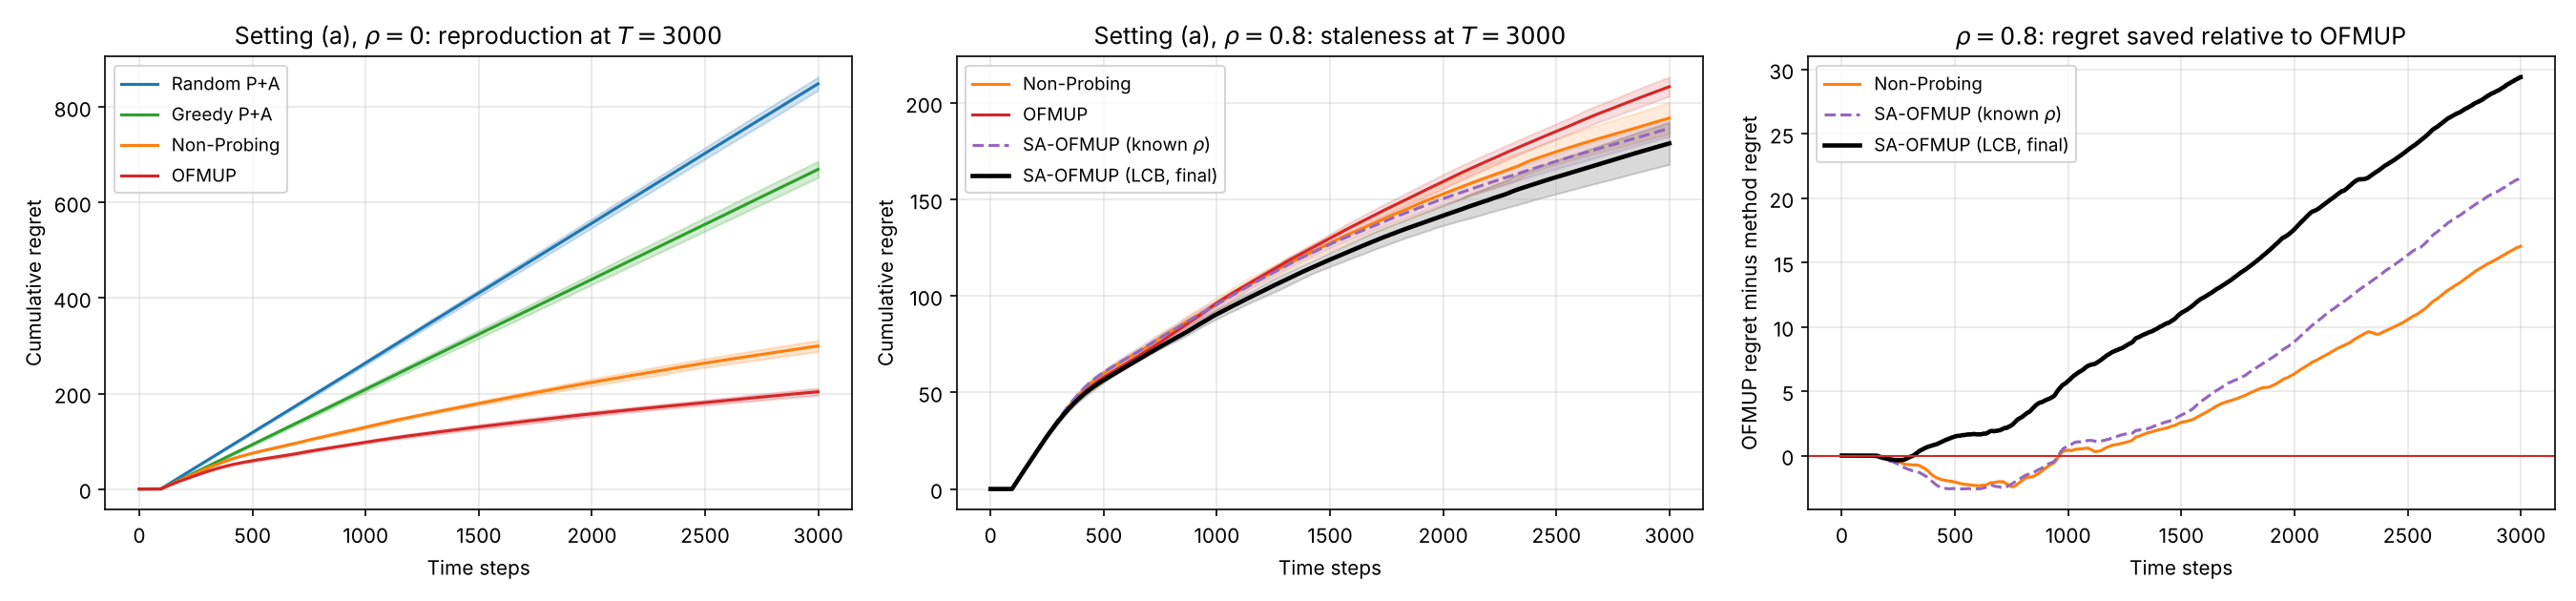
\includegraphics[width=\textwidth]{results/long_T3000.png}
\caption{Results at the original horizon $T=3000$ in setting (a), mean over 3
seeds (one s.d.\ shaded). Left: reproduction at $\rho=0$
(Table~\ref{tab:repro3000}). Middle: staleness at $\rho=0.8$
(Table~\ref{tab:long}). Right: regret saved relative to OFMUP at $\rho=0.8$
(OFMUP's regret minus the method's, paired by seed). SA-OFMUP (LCB, final)
builds its lead over SA-OFMUP (known $\rho$) over roughly the first 1500 rounds,
while it is still probing; the lead then levels off at about 8 regret points,
a one-time gain, whereas both methods keep gaining on OFMUP. Colours are
consistent across all figures.}
\label{fig:long}
\end{figure*}

\section{Analysis of the OFMUP Formulation}
\label{sec:findings}

My reproduction suggests the following points in \citet{xu2026fair}, which I
recommend checking against the full version \citep{xu2025fairarxiv}.
\begin{enumerate}
\item \textbf{Infeasible constraints.} The requirement $\sum_j\pi_{j,a}\le1$
      cannot be met in any of the original experimental settings
      ($M>A$); its experiments presumably used a relaxed model that
      is not described.
\item \textbf{Double counting.} At $\rho=0$ a pull from a just-probed arm
      returns the probed draw (otherwise \eqref{eq:nsw} would not be the
      realised payoff), yet lines 13 and 16 of Xu et al.'s Algorithm~2 both record it.
\item \textbf{Scale mismatch in Xu et al.'s Algorithm~1.} Lines 9 and 11 compare the
      log-scale surrogate $f_{\mathrm{upper}}$ with NSW-scale values.
\item \textbf{$\phi$ is irrelevant to the greedy choice.} Because $\phi$ is
      strictly increasing, the greedy chain is the chain of $g$; the
      construction matters only for the submodularity argument.
\item \textbf{$\phi$ as a maximum of tangents.} \citet{xu2026fair} define
      $\phi(z)=\max_i T_{\tau_i}(z)$ and calls it concave; a maximum of affine
      functions is convex. The concave upper envelope required by the proof
      is the \emph{minimum} of the tangents.
\item \textbf{Lemma 5.} As written, Lemma~5 states that for any probing set $S$,
      \begin{align*}
        \mathcal{R}(S)&=(1-\alpha(|S|))\,\E_R[\NSW(S,R,\mu,\pi^\ast(S))]\\
        &\le(1-\alpha(|S|))(g(S)+h(S)).
      \end{align*}
      Take two agents and two arms with
      $\mu_{1,1}=\mu_{2,2}=1$ and $\mu_{1,2}=\mu_{2,1}=0$ (deterministic
      rewards), and $S=\{1\}$. Then $g(S)=0$ because agent~2 earns nothing on
      arm~1, and $h(S)=0$ because agent~1 earns nothing on arm~2, but
      $\mathcal{R}(S)=(1-\alpha(1))\cdot1\cdot1>0=(1-\alpha(1))(g(S)+h(S))$.
      Unless the appendix adds assumptions, the stated upper bound fails.
\item \textbf{Position of the maximisation in $g(S)$.} With the maximum outside
      the expectation, as written, $g(S)$ does not depend on the probe outcomes
      at all (for independent agents it is the NSW of the means on $S$); the
      value of information enters only through $\mathcal{R}(S)$.
\end{enumerate}

\section{Limitations and Future Work}
This work has four main limitations. First, my horizon and seed count are
below those of \citet{xu2026fair}: the sweeps
use $T=\TT$, and all results use three seeds, so the gains at $\rho=0.8$ are
indications rather than a confirmed effect size; confirming them with more
seeds is the first item of future work. The code supports the full setting.
Second, the staleness model is all-or-nothing; a graded model (demand depletion, or, in
ridesharing, $\rho$ increasing with the driver's distance,
$\rho_{j,a}=1-e^{-d_{j,a}/\tau}$, natural for the taxi setting) is a natural
extension and would likely show larger regret gains. Third, Xu et al.'s Algorithm~1 ignores
the learning value of probes; adding an exploration bonus to the probe-selection
score is a promising complement to SA-OFMUP. Fourth, the regret analysis of
SA-OFMUP is a proof direction, not a theorem: the estimation error of $\rhat$ and its effect
on probe selection remain to be bounded. In addition, I did not run the NYC-taxi
experiment of \citet{xu2026fair}; the code supports it, but any staleness
experiment on historical data would be semi-synthetic, since the data cannot
reveal what a driver would have found after a hypothetical delay.

\section{Conclusion}
I reproduced the fair probing framework of \citet{xu2026fair}, documented the
decisions needed to run it, and identified several issues in its formulation.
My extension, SA-OFMUP, removes the unrealistic assumption that a probe is
still valid when an agent reaches the probed arm. It is exact for the
original product-of-expected-utilities objective, learns the
staleness rate online with an estimator that is consistent under stated
conditions (proof sketch), plans with a lower
confidence bound to avoid locking in on early noise, reduces exactly to OFMUP
(with the counting fix) when probes are reliable, and, in my experiments,
reduces probing and regret when they are not.

\bibliographystyle{aaai2026}
\bibliography{references}

\end{document}
